\documentclass[11pt,a4paper]{article}\usepackage[utf8]{inputenc}

\usepackage[T1]{fontenc}
\usepackage{tgpagella}
\usepackage[spanish]{babel}
\usepackage{geometry}
\usepackage{graphicx}
\usepackage{booktabs}
\usepackage{array}
\usepackage{xcolor}
\usepackage{titlesec}
\usepackage{fancyhdr}
\usepackage[parfill]{parskip}
\usepackage[expansion=false]{microtype}
\usepackage{hyperref}
\usepackage{setspace}
\usepackage{needspace}

\geometry{top=3.0cm,bottom=3.0cm,left=3.5cm,right=3.5cm}
\setlength{\parskip}{0.65em}
\setlength{\parindent}{0em}

\definecolor{azulai}{RGB}{30,80,140}
\definecolor{doradoai}{RGB}{140,90,0}
\definecolor{grisai}{RGB}{70,70,70}

\titleformat{\section}{\Large\bfseries\color{azulai}}{}{0em}{}[{\color{azulai}\titlerule[0.5pt]\nopagebreak[4]}]
\titlespacing*{\section}{0pt}{1.8em}{0.8em}
\titleformat{\subsection}{\large\bfseries\color{doradoai}}{}{0em}{}[{\nopagebreak[4]}]
\titlespacing*{\subsection}{0pt}{1.4em}{0.5em}
\titleformat{\subsubsection}{\normalsize\bfseries\color{grisai}}{}{0em}{}[{\nopagebreak[4]}]
\titlespacing*{\subsubsection}{0pt}{1.0em}{0.3em}

\pagestyle{fancy}\fancyhf{}
\rhead{\textcolor{grisai}{\small Raquel Pain — Arquitectura Interna}}
\lhead{\textcolor{grisai}{\small Carta Natal Completa}}
\cfoot{\textcolor{grisai}{\small\thepage}}
\renewcommand{\headrulewidth}{0.3pt}

\hypersetup{colorlinks=true,linkcolor=azulai,urlcolor=azulai}
\setstretch{1.45}
\tolerance=1500
\emergencystretch=4em

\begin{document}

% ── Portada ──────────────────────────────────────────────────────────────────
\begin{titlepage}
  \centering
  \vspace*{1.5cm}
  {\Huge\bfseries\color{azulai} Carta Natal Completa}\\[0.5cm]
  {\large\color{grisai} Arquitectura Interna}\\[0.3cm]
  {\small\itshape\color{grisai} Un método para sostener cuerpo, energía y vida con coherencia}\\[2cm]
  {\huge\color{doradoai} Raquel Pain}\\[1.5cm]
  {\Large 07/03/1985 \quad 18:20}\\[0.3cm]
  {\Large Pamplona, España}\\[0.3cm]
  {\normalsize Lat: 42.8157° \quad Lon: -1.6522° \quad UTC+01:00}\\[0.3cm]
  {\normalsize Ascendente: Virgo 9°36' \quad
    MC: Géminis 5°37'}\\[2.5cm]
  \vfill
  {\small Generado el 14/05/2026}
\end{titlepage}

\tableofcontents
\newpage

% ── Rueda ─────────────────────────────────────────────────────────────────────
\section{Carta Natal}
\begin{figure}[h!]
  \centering
  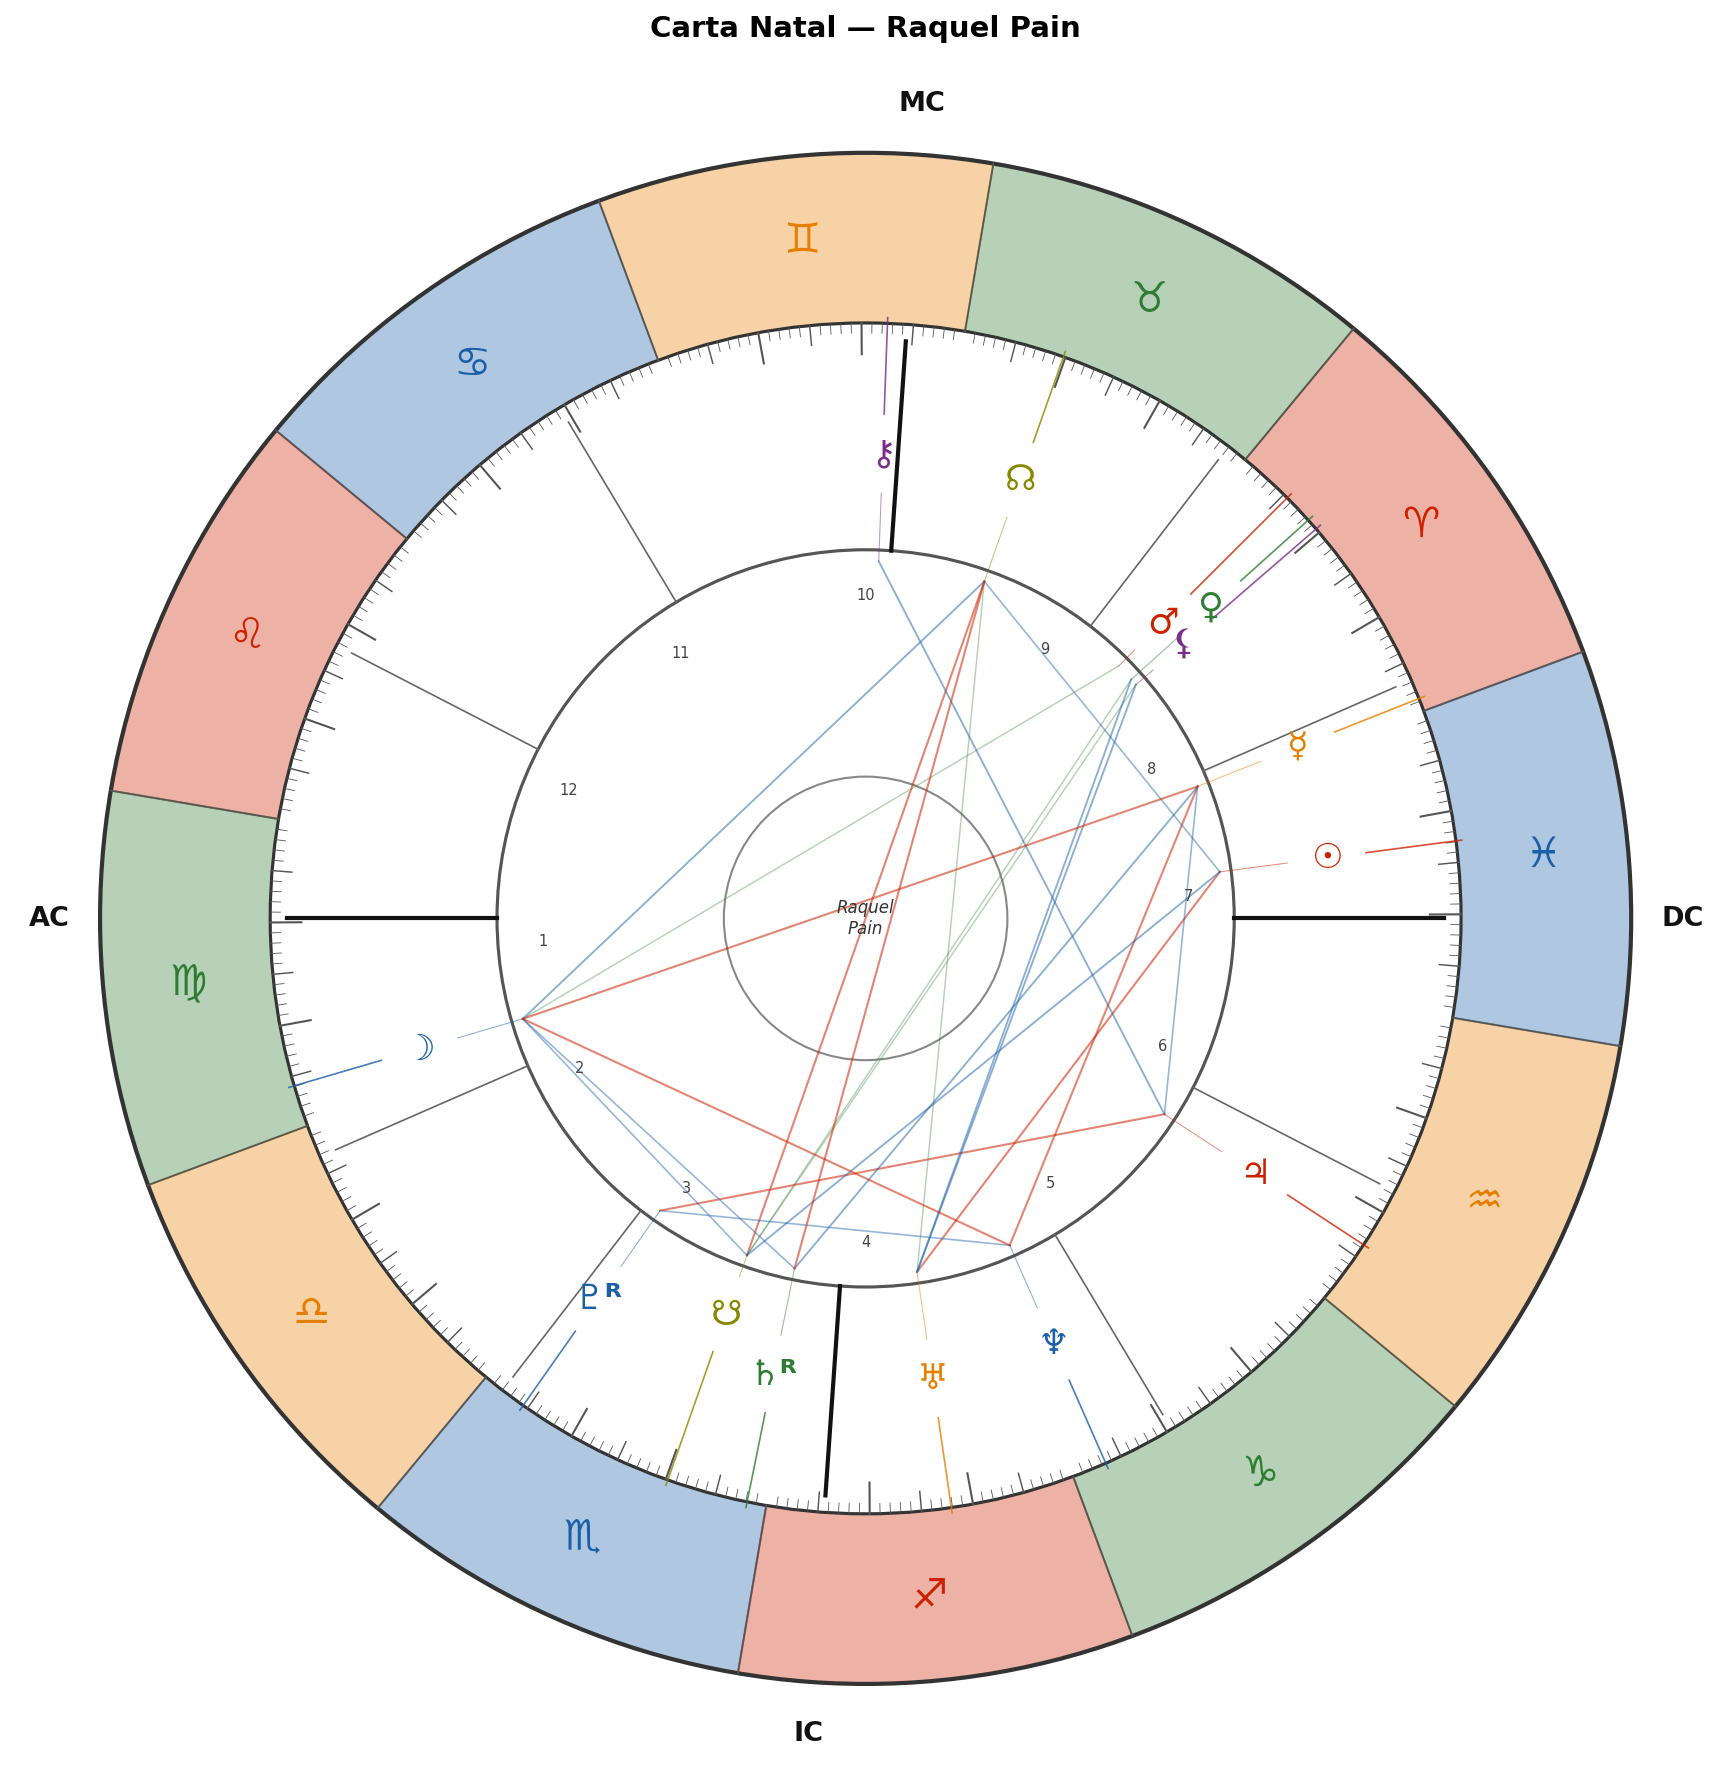
\includegraphics[width=0.90\textwidth]{Raquel_Pain_AI_rueda.png}
  \caption{Carta natal de Raquel Pain — 07/03/1985 18:20 — Pamplona, España}
\end{figure}

\newpage

% ── Tabla de posiciones ───────────────────────────────────────────────────────
\section{Posiciones Planetarias}

\begin{center}
\begin{tabular}{llrrlll}
  \toprule
  \textbf{Planeta} & \textbf{Signo} & \textbf{Grado} & \textbf{Casa} &
  \textbf{Elemento} & \textbf{R} \\
  \midrule
  Sol & Piscis & 17°05' & 7 & Agua &  \\
  Luna & Virgo & 25°56' & 1 & Tierra &  \\
  Mercurio & Aries & 1°17' & 7 & Fuego &  \\
  Venus & Aries & 21°35' & 8 & Fuego &  \\
  Marte & Aries & 24°32' & 8 & Fuego &  \\
  Júpiter & Acuario & 6°22' & 5 & Aire &  \\
  Saturno & Escorpio & 28°08' & 3 & Agua & R \\
  Urano & Sagitario & 17°53' & 4 & Fuego &  \\
  Neptuno & Capricornio & 3°24' & 4 & Tierra &  \\
  Plutón & Escorpio & 4°30' & 3 & Agua & R \\
  Quirón & Géminis & 7°30' & 10 & Aire &  \\
  Lilith & Aries & 20°27' & 8 & Fuego &  \\
  Nodo Norte & Tauro & 20°12' & 9 & Tierra &  \\
  Nodo Sur & Escorpio & 20°12' & 3 & Agua &  \\
  \bottomrule
\end{tabular}
\end{center}

\vspace{0.5cm}
\begin{itemize}
  \item \textbf{Ascendente:} Virgo 9°36'
  \item \textbf{Medio Cielo:} Géminis 5°37'
\end{itemize}

\newpage

% ── Interpretación ────────────────────────────────────────────────────────────
\section{Interpretación — Arquitectura Interna}

\begin{center}
{\small\itshape
No se trata de definirte. Se trata de observar cómo se organiza tu energía,\
dónde puedes perder equilibrio y qué apoyos te ayudan a sostenerte.
}
\end{center}

\vspace{0.5cm}

\subsection{1. Visión General}

Tu carta muestra la siguiente distribución de elementos: Fuego 6.5, Tierra 5, Aire 1, Agua 4. Fuego (vitalidad, iniciativa, necesidad de sentido y movimiento hacia la acción): ahí está el peso de tu carta. Es el registro desde el que tu energía se activa con más fluidez y sin esfuerzo consciente. Aire (desapego, análisis, pensamiento relacional y capacidad de perspectiva) está poco representado en tu carta. Ese territorio puede pedirte un esfuerzo consciente, especialmente cuando la presión sube.  Tu Medio Cielo en Géminis: La comunicación, el aprendizaje y la capacidad de moverte entre distintos temas o personas. Funcionas bien en entornos donde la palabra, el intercambio y la circulación de ideas son importantes.

\subsection{2. Ejes Principales}

\subsubsection*{Sol en Piscis — Casa 7}
Tu Sol en Piscis funciona con mucha apertura al entorno. Percibes matices, estados y necesidades que no siempre están expresados de forma clara. Eso puede darte sensibilidad y facilidad para conectar con lo que ocurre alrededor, pero también puede hacer que te adaptes demasiado. La dificultad aparece cuando no hay límites suficientes: puedes perder claridad sobre lo que quieres tú. En Casa 7, muchas de las cosas importantes de tu vida se activan a través del vínculo con otras personas. Las relaciones, asociaciones y encuentros significativos suelen tener un impacto directo en cómo te ves. El contacto con el la otra persona te ayuda a reconocer aspectos propios que quizá no verías por tu cuenta. El riesgo aparece cuando adaptarte al vínculo pesa más que sostener tu propia posición.

\subsubsection*{Luna en Virgo — Casa 1}
Tu Luna en Virgo procesa las emociones a través del análisis y la búsqueda de orden. Sueles observar y evaluar constantemente cómo estás. Eso puede ser útil o puede convertirse en un obstáculo cuando la emoción necesita ser sentida antes de ser analizada. La claridad en el entorno cotidiano y la sensación de utilidad funcionan como suelo. En Casa 1, tus necesidades emocionales tienden a expresarse directamente a través del cuerpo y la presencia. Lo que sientes suele reflejarse rápidamente en el cuerpo, la postura o la forma de reaccionar al entorno.

\subsubsection*{Ascendente Virgo}
Tu Ascendente en Virgo hace que los demás te vean como una persona analítica, discreta y orientada al detalle. Observa y evalúa antes de participar. Puede haber una distancia inicial que no refleja la calidez que aparece cuando coges confianza. Su regente es Mercurio, en Aries y Casa 7. El Ascendente toma el tono de Aries: directa, rápida y orientada a la acción. Esa energía opera principalmente desde las relaciones importantes, las asociaciones y el vínculo con la otra persona.

\subsubsection*{Grados finales de signo}
Los grados finales de signo muestran funciones que están cerca de un punto de cierre, maduración o cambio de modo. No se interpretan como destino ni como algo negativo, sino como zonas donde la energía del signo aparece muy concentrada. Puede haber más intensidad, menos margen para funcionar de forma automática y una sensación interna de que una forma antigua de responder ya no se sostiene igual.

También aparecen posiciones en grado previo al anarético. No tienen la misma presión que el grado 29, pero sí muestran zonas donde ya existe mucha maduración acumulada y cierta necesidad de revisar cómo se está usando esa energía.

Saturno en Escorpio 28°08', Casa 3 aparece en grado previo al anarético. La estructura, la responsabilidad y el límite aparecen muy intensificados. Puede haber una gran capacidad para sostener, resistir y hacerse cargo, pero también cansancio profundo de funcionar desde exigencia. Puedes seguir adelante incluso cuando el cuerpo ya está pidiendo pausa. El aprendizaje está en comprender que parar también forma parte de la estructura, no es una pérdida de control.

Cuando varios puntos de la carta están al final de un signo, suele haber menos sensación de margen interno o de estabilidad automática. Las cosas tienden a vivirse con más intensidad, más urgencia o con la sensación de estar siempre cerca de un cambio importante. No significa que haya más dificultad, sino que esas zonas piden más cuerpo, más pausa y más consciencia antes de seguir respondiendo desde el patrón habitual.



\subsection{3. Organización de la Energía}

Tu Mercurio en Aries piensa rápido y va directo a la acción. Captas lo esencial con facilidad, pero puede costarte detenerte en matices o escuchar demasiado tiempo antes de responder. Te ayuda dejar un pequeño espacio entre la idea y la reacción. En Casa 7, el pensamiento se activa mucho a través de otras personas. Las conversaciones, los vínculos y los intercambios importantes estimulan tu forma de pensar y ayudan a ordenar ideas. Tu Venus en Aries se vincula con impulso, franqueza y necesidad de movimiento. Te atraen los vínculos vivos, donde hay deseo, iniciativa y espacio para actuar. El riesgo aparece cuando la intensidad inicial baja y cuesta sostener ritmos más lentos. En Casa 8, los vínculos necesitan profundidad, confianza y sensación de entrega real. Las relaciones superficiales suelen dejarte vacío cuando algo importa de verdad. Tu Marte en Aries actúa rápido, con iniciativa y poca espera. Cuando algo se activa, necesitas moverte o intervenir. El riesgo aparece cuando la acción se adelanta a la evaluación y terminas gastando fuerza antes de tener una dirección clara. En Casa 8, la acción aparece con mucha fuerza en situaciones intensas, límites o momentos de crisis. Hay capacidad de resistencia y dificultad para hacer las cosas a medias cuando algo importa.

\subsection{4. Estructura y Tensión}

\subsubsection*{Concentración de energía}

Hay una concentración notable en Casa 8: Venus, Marte y Lilith. Cuando varios planetas ocupan la misma casa, esa área absorbe buena parte de la actividad vital. En esta carta, el foco de los vínculos intensos, las pérdidas y las situaciones difíciles de controlar funciona como núcleo central: ahí se acumula la presión, la demanda es mayor y también hay más recursos disponibles para operar. No es necesariamente un conflicto, pero sí un punto de alta intensidad sostenida.

También hay una concentración significativa en Casa 3: Saturno, Plutón y Nodo Sur. En este caso, el foco se desplaza hacia la comunicación, el aprendizaje y el entorno cercano. Es un ámbito donde la exigencia aumenta, donde se concentra parte de la presión y donde también existe capacidad real de sostener procesos importantes. Tampoco es en sí un problema, pero sí un área de intensidad mantenida.



Los aspectos aparecen organizados en dos niveles. Los aspectos exactos (orbe igual o menor a 1°) suelen sentirse de forma más inmediata y constante en la vida cotidiana. Los aspectos estructurales tienen un orbe más amplio, pero siguen describiendo dinámicas importantes que se repiten a lo largo de la vida.



\Needspace{8\baselineskip}
\subsubsection*{Aspectos exactos}
No aparecen aspectos exactos especialmente fuertes dentro del orbe definido para esta lectura. Eso no significa ausencia de tensión o profundidad, sino que gran parte de las dinámicas importantes de la carta se construyen de forma más amplia y progresiva. En este caso, cobran más importancia los aspectos estructurales y la combinación general de posiciones.

\Needspace{8\baselineskip}
\subsubsection*{Aspectos estructurales}
\Needspace{7\baselineskip}
\subsubsection*{Venus (Casa 8) trígono Urano (Casa 4) --- orbe 3.7\textdegree}
El trígono Venus-Urano da una forma relacional independiente y poco convencional. Sueles necesitar libertad dentro de los vínculos y te atraen relaciones donde haya autenticidad, diferencia o espacio propio. Lo demasiado previsible puede apagarte, pero lo inestable tampoco siempre te sostiene. La clave está en diferenciar libertad real de distancia emocional.



\subsection{5. Sostén y Equilibrio}

Tu Quirón en Géminis, Casa 10, señala una zona sensible relacionada con la comunicación, el aprendizaje y la capacidad de expresarte con libertad. Puede que hayas sentido que tus palabras no eran escuchadas o que pensar diferente generaba incomodidad. Esto suele notarse especialmente en la vocación, la responsabilidad y el reconocimiento. No significa que tengas límites en ese terreno, pero sí que probablemente necesites más tiempo, cuidado o consciencia para sentir estabilidad ahí.

\vspace{0.3cm}
Tu Nodo Sur en Escorpio, Casa 3, muestra una tendencia a moverte desde la intensidad constante, el control o la dificultad para soltar situaciones desgastadas, especialmente en la comunicación y el entorno cercano. Suele ser una forma de funcionar conocida o automática para ti. Tu Nodo Norte en Tauro, Casa 9, señala la necesidad de construir estabilidad real, paciencia y una relación más sencilla con lo concreto, especialmente en el aprendizaje, las creencias y la necesidad de ampliar horizontes. No se trata de rechazar lo anterior, sino de ampliar tu forma habitual de responder.

\vspace{0.3cm}
En tu carta hay poca presencia de Aire. Cuando aparece saturación, bloqueo o sensación de desorganización interna, suele ayudarte volver a espacios relacionados con la perspectiva, el espacio mental y las conversaciones que ordenan. Eso puede darte más estabilidad y ayudarte a recuperar claridad.

\subsection{6. Orientación}

\subsubsection*{Qué observar}
Tu Ascendente en Virgo describe la forma en que otras personas suelen percibirte al principio. Eso no siempre coincide con cómo vives las cosas internamente o con las tensiones más importantes de tu carta. Cuando hay demasiada distancia entre lo que muestras y lo que realmente te ocurre, aparece desgaste.

\subsubsection*{Qué puede desestabilizar}
Hay ciertas tensiones en tu carta que pueden activarse con bastante fuerza: Nodo Norte-Nodo Sur, Lilith-Nodo Sur, Sol-Urano. Cuando varias coinciden al mismo tiempo, puede aparecer sensación de saturación, reacción excesiva o dificultad para mantener claridad.

\subsubsection*{Qué estructura y sostiene}
Tu Sol en Piscis, Casa 7, muestra un terreno importante de estabilidad para ti. Cuando tu forma de actuar está alineada con lo que realmente valoras, suele aparecer más claridad y menos dispersión.

\subsubsection*{Orientación práctica}
Una orientación práctica: en tu carta hay poco Aire. Cuando las emociones o las tensiones aumentan, puede costarte tomar distancia y ordenar lo que te ocurre. Escribir, hablar con alguien de confianza o darte tiempo antes de reaccionar puede ayudarte mucho más de lo que parece.

\vspace{1cm}
\begin{center}
{\small\itshape\color{grisai}
La astrología se usa aquí como lenguaje simbólico de observación, no como una definición de quién eres.\\
Esta interpretación es tu mapa de posibilidades, no tu destino fijo.
}
\end{center}

\end{document}
